% !TEX encoding = UTF-8 Unicode
\documentclass[]{beamer}
\setbeamertemplate{caption}[numbered]
\setbeamertemplate{caption label separator}{: }
\setbeamercolor{caption name}{fg=normal text.fg}
\beamertemplatenavigationsymbolsempty
\usepackage{lmodern}
\usepackage{amssymb,amsmath}
\usepackage{ifxetex,ifluatex}
\usepackage{fixltx2e} % provides \textsubscript
\ifnum 0\ifxetex 1\fi\ifluatex 1\fi=0 % if pdftex
  \usepackage[T1]{fontenc}
  \usepackage[utf8]{inputenc}
\else % if luatex or xelatex
  \ifxetex
    \usepackage{mathspec}
  \else
    \usepackage{fontspec}
  \fi
  \defaultfontfeatures{Ligatures=TeX,Scale=MatchLowercase}
\fi
% use upquote if available, for straight quotes in verbatim environments
\IfFileExists{upquote.sty}{\usepackage{upquote}}{}
% use microtype if available
\IfFileExists{microtype.sty}{%
\usepackage{microtype}
\UseMicrotypeSet[protrusion]{basicmath} % disable protrusion for tt fonts
}{}
\newif\ifbibliography
\hypersetup{
            pdftitle={A Data-Driven Early Warning System for Mining Accidents},
            pdfborder={0 0 0},
            breaklinks=true}
\urlstyle{same}  % don't use monospace font for urls
\usepackage{graphicx,grffile}
\makeatletter
\def\maxwidth{\ifdim\Gin@nat@width>\linewidth\linewidth\else\Gin@nat@width\fi}
\def\maxheight{\ifdim\Gin@nat@height>\textheight0.8\textheight\else\Gin@nat@height\fi}
\makeatother
% Scale images if necessary, so that they will not overflow the page
% margins by default, and it is still possible to overwrite the defaults
% using explicit options in \includegraphics[width, height, ...]{}
\setkeys{Gin}{width=\maxwidth,height=\maxheight,keepaspectratio}

% Prevent slide breaks in the middle of a paragraph:
\widowpenalties 1 10000
\raggedbottom

\AtBeginPart{
  \let\insertpartnumber\relax
  \let\partname\relax
  \frame{\partpage}
}
\AtBeginSection{
  \ifbibliography
  \else
    \let\insertsectionnumber\relax
    \let\sectionname\relax
    \frame{\sectionpage}
  \fi
}
\AtBeginSubsection{
  \let\insertsubsectionnumber\relax
  \let\subsectionname\relax
  \frame{\subsectionpage}
}

\setlength{\parindent}{0pt}
\setlength{\parskip}{6pt plus 2pt minus 1pt}
\setlength{\emergencystretch}{3em}  % prevent overfull lines
\providecommand{\tightlist}{%
  \setlength{\itemsep}{0pt}\setlength{\parskip}{0pt}}
\setcounter{secnumdepth}{0}
\usepackage{cris_style,l16cn}

% http://rmarkdown.rstudio.com/articles_beamer.html
\AtBeginPart{}
\AtBeginSection{}
\AtBeginSubsection{}
\AtBeginSubsubsection{}
\setlength{\emergencystretch}{0em}
\setlength{\parskip}{0pt}

%% http://stackoverflow.com/questions/38323331/code-chunk-font-size-in-beamer-with-knitr-and-latex
%%% change fontsize of R code
%\let\oldShaded\Shaded
%\let\endoldShaded\endShaded
%\renewenvironment{Shaded}{\footnotesize\oldShaded}{\endoldShaded}

%% change fontsize of output
\let\oldverbatim\verbatim
\let\endoldverbatim\endverbatim
\renewenvironment{verbatim}{\footnotesize\oldverbatim}{\endoldverbatim}

\title[Mining Accident Data Analysis]{A Data-Driven Early Warning System for Mining Accidents}
\author[Luo et al.]{Yu Luo, Ashutosh Nanda, Shivaram Rajgopal, Vinay Ramesh,\\
Zhizun Zhang, Catherine Zhao, and Venkat Venkatasubramanian}
\institute[Columbia University]{Chemical Engineering, Computer Science, and Business School\\
Columbia University}
\date{3/27/2017}

\begin{document}
\frame{\titlepage}

\begin{frame}
\tableofcontents[hideallsubsections]
\end{frame}

\begin{frame}{Complex, Resilient, Intelligent Systems (CRIS Lab)}

\begin{figure}[htbp]
\centering
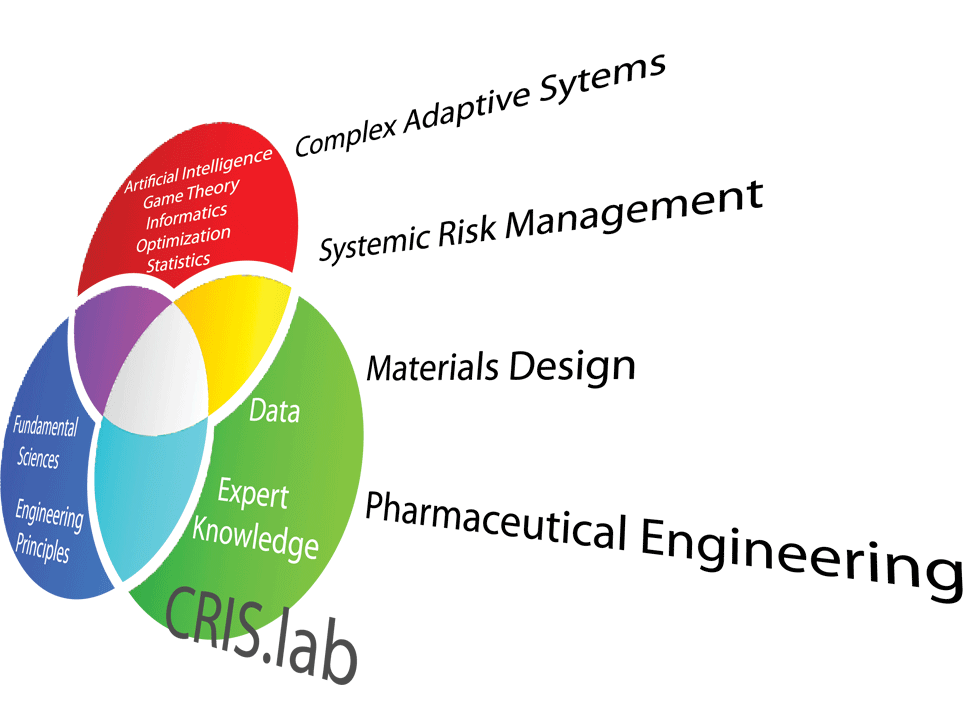
\includegraphics{CrisResearch720.png}
\caption{CRIS Lab}
\end{figure}

\end{frame}

\section{Mine Safety: A Data-Driven
Approach}\label{mine-safety-a-data-driven-approach}

% !TEX root = presentation_slides.tex

%\placelogofalse
\begin{frame}{Systemic Risk}
\begin{columns}[c]
	\column{0.475\linewidth}
		\begin{itemize}[<+->]
		\item Systemic disasters
		\begin{itemize}
			\item SARS (2003)
			\item Northeast Blackout (2003)
			\item Subprime Crisis (2008)
			\item Deepwater Horizon
			%Oil Spill 
			(2010)
		\end{itemize}
		\item Emerging systemic risks
		\begin{itemize}
			\item Climate change
			\item Income/wealth inequality
			\item Cyber-physical security
%			\item Technological singularity
		\end{itemize}
		\item Fast-paced and connected
		\item Prevent systemic disasters
		\item Go beyond one-off accidents
		\end{itemize}
	\column{0.525\linewidth}
	   \onslide<2->
	   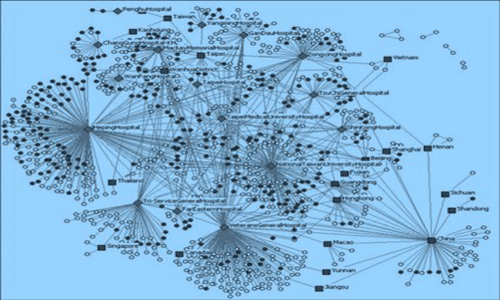
\includegraphics[width = .5\linewidth]{fig/wide_SARS.png}
	   \onslide<7->
	   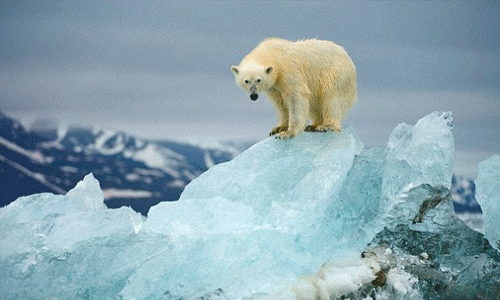
\includegraphics[width = .5\linewidth]{fig/wide_polarbear.png}\\%http://i.dailymail.co.uk/i/pix/2014/09/09/1410255561618_wps_15_Spitsbergen_Norway_Polar_.jpg
	   \onslide<3->
	   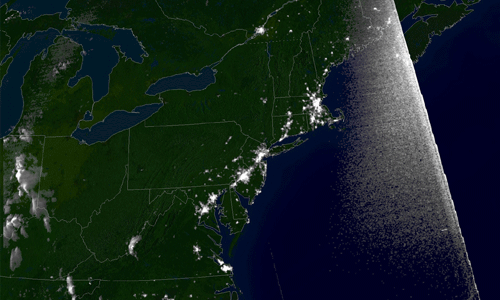
\includegraphics[width = .5\linewidth]{fig/wide_NEB.png}
	   \onslide<8->
	   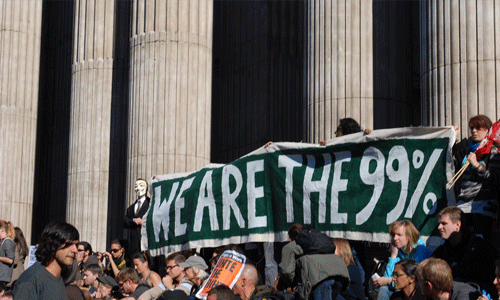
\includegraphics[width = .5\linewidth]{fig/wide_99.png}\\%https://c1.staticflickr.com/7/6055/6247188828_305409d56a_b.jpg
	   \onslide<4->
	   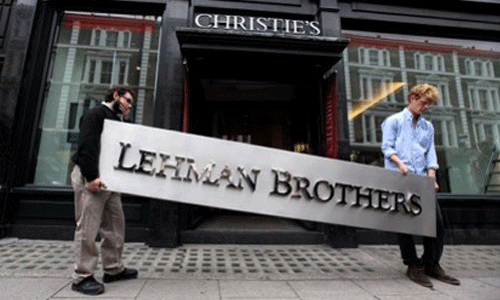
\includegraphics[width = .5\linewidth]{fig/wide_FIN.png}
	   \onslide<9->
	   
\includegraphics[width = .5\linewidth]{fig/wide_cyber.png}\\%https://c1.staticflickr.com/9/8604/16042227002_1d00e0771d_b.jpg
	   \onslide<5->
	   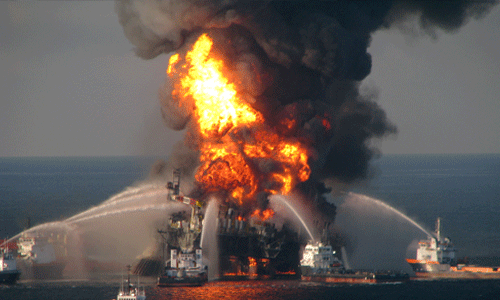
\includegraphics[width = .5\linewidth]{fig/wide_BP.png}
%	   \onslide<10->
%	   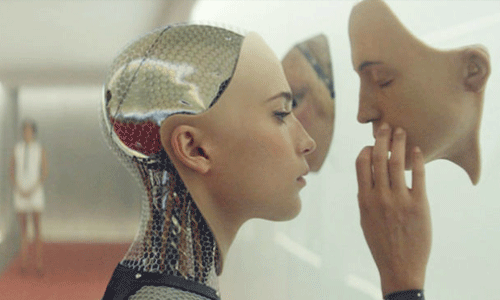
\includegraphics[width = .5\linewidth]{fig/wide_exmachina.png}%https://c1.staticflickr.com/1/569/20167701293_e3ed4b066f_b.jpg
\end{columns}
\end{frame}

%\begin{frame}{Systemic Risk}
%\begin{itemize}[<+->]
%\tightlist
%\item
%  Systemic disasters
%
%  \begin{itemize}[<+->]
%  \tightlist
%  \item
%    SARS (2003)
%  \item
%    Northeast Blackout (2003)
%  \item
%    Subprime Crisis (2008)
%  \item
%    Deepwater Horizon Oil Spill (2010)
%  \end{itemize}
%\item
%  Emerging systemic risks
%
%  \begin{itemize}[<+->]
%  \tightlist
%  \item
%    Climate change
%  \item
%    Income/wealth inequality
%  \item
%    Cyber-physical security
%  \item
%    Technological singularity
%  \end{itemize}
%\item
%  Fast-paced and connected
%\item
%  Prevent systemic disasters
%\item
%  Analyze systemic risk: go beyond one-off accidents
%\end{itemize}
%
%\end{frame}

\begin{frame}{Upper Big Branch Mine Disaster (2010)}

\begin{itemize}[<+->]
\tightlist
\item
  April 5, 2010, Raleigh County, West Virginia, owned by Massey Energy
\item
  29 deaths, the worst mining in the United States since 1970
\item
  MSHA cites corporate culture as root cause of Upper Big Branch Mine
  disaster
\end{itemize}

\end{frame}

\begin{frame}{Sago Mine Disaster (2006)}

\begin{itemize}[<+->]
\tightlist
\item
  January 2, 2006, Sago, West Virginia, owned by Anker West Virginia
  Mining
\item
  13 miners were trapped for nearly two days; only one survived
\item
  Fatality number was exceeded by the Upper Big Branch Mine disaster
\item
  MSHA reports prior history of safety violations and fatalities
\end{itemize}

\end{frame}

\begin{frame}{Mine Safety and Health Administration (MSHA)}

\begin{itemize}[<+->]
\tightlist
\item
  Formed in 1977, agency of the U.S. Department of Labor
\item
  Mission

  \begin{itemize}[<+->]
  \tightlist
  \item
    Prevent death, illness, and injury from mining
  \item
    Promote safe and healthful workplaces for U.S. miners
  \item
    Develop and enforce safety and health rules
  \item
    Provide technical, educational, and other types of assistance
  \end{itemize}
\item
  A constantly improving industry in terms of safety
\end{itemize}

\end{frame}

\begin{frame}{Fatality Trend Since 1983}

\begin{center}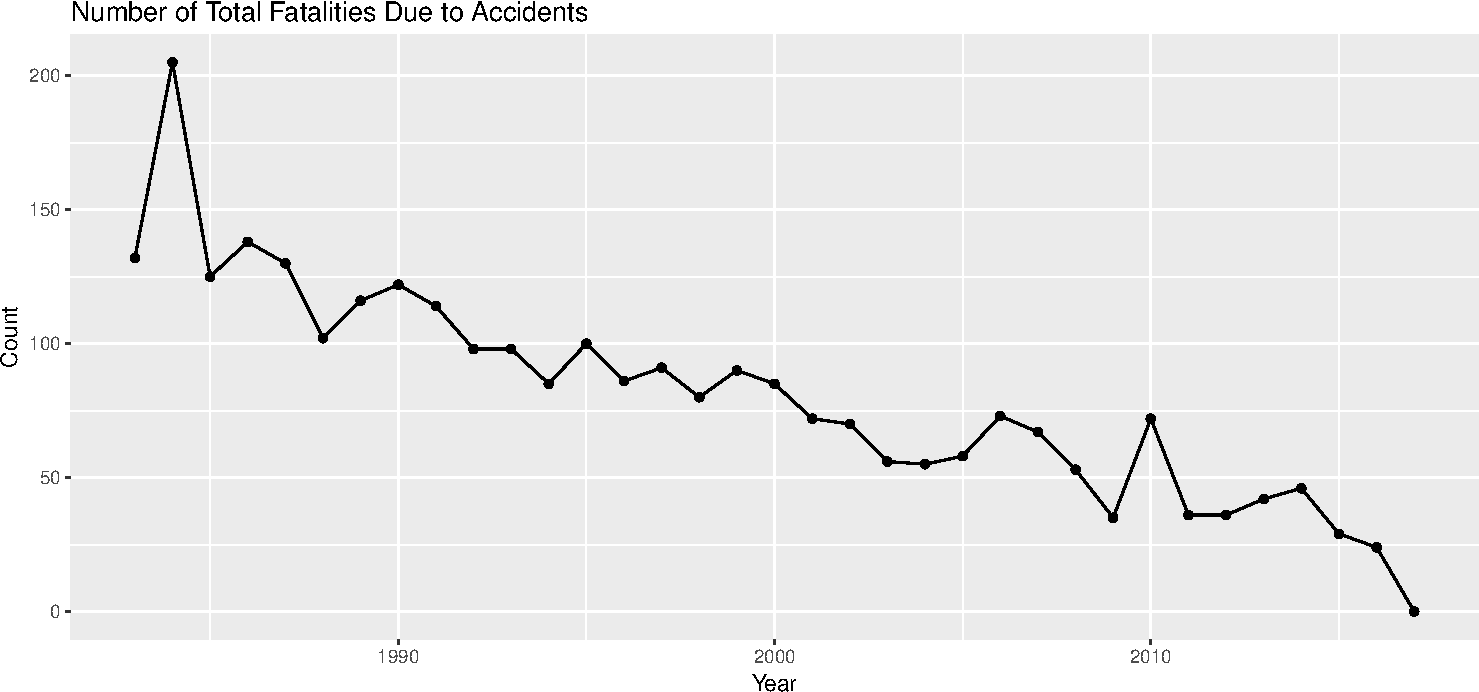
\includegraphics{presentation_slides_files/figure-beamer/fatality trend-1} \end{center}

\end{frame}

\begin{frame}{Can We Further Improve Mine Safety?}

\begin{itemize}[<+->]
\tightlist
\item
  Process MSHA safety data
\item
  Understand the underlying causal relationships
\item
  Develop early warning systems based on past behaviors
\item
  Credit rating/score analogy

  \begin{itemize}[<+->]
  \tightlist
  \item
    Predict default probability within 18 months
  \item
    Accidents: defaults a month or a year prior to application
  \item
    Violations: missed payments, late payments, etc.
  \end{itemize}
\item
  Can we develop a ``credit score'' for mine safety?
\end{itemize}

\end{frame}

\section{Methods: Data Sources and Model
Preliminaries}\label{methods-data-sources-and-model-preliminaries}

\begin{frame}{Department of Labor Enforcement Data}

\begin{itemize}[<+->]
\tightlist
\item
  Link: \url{https://enforcedata.dol.gov/views/data_catalogs.php}
\item
  Updated daily or weekly
\item
  Publicly available

  \begin{itemize}[<+->]
  \tightlist
  \item
    Department of Labor: MSHA, OSHA, etc.
  \item
    Other departments: EPA, FDA, DOJ, etc.
  \end{itemize}
\end{itemize}

\end{frame}

\begin{frame}{MSHA Data: Sources}

\begin{itemize}[<+->]
\tightlist
\item
  Mine accidents table: ``msha\_accident.csv''

  \begin{itemize}[<+->]
  \tightlist
  \item
    681,386 rows
  \item
    Retrieved 1/26/2017, from
    \url{https://enforcedata.dol.gov/views/data_summary.php}
  \end{itemize}
\item
  MSHA assessed violations table: ``AssessedViolations.csv''

  \begin{itemize}[<+->]
  \tightlist
  \item
    2,169,804 rows
  \item
    Retrieved 12/10/2016, from
    \url{https://arlweb.msha.gov/OpenGovernmentData/OGIMSHA.asp}
  \end{itemize}
\end{itemize}

\end{frame}

\begin{frame}[fragile]{MSHA Data: Advantages}

\begin{itemize}[<+->]
\tightlist
\item
  Each mine has a unique mine ID, e.g., Upper Big Branch (4608436)
\item
  Rich details: e.g., classification, description, and severity
\item
  Selected attributes from the accidents table (omitting 42 attributes)
%\end{itemize}

\begin{verbatim}
##  [1] "mine_id"          "controller_id"    "cal_yr"          
##  [4] "cal_qtr"          "ai_dt"            "inj_degr_desc"   
##  [7] "ai_class_desc"    "ai_occ_desc"      "ai_acty_desc"    
## [10] "exper_tot_calc"   "exper_mine_calc"  "exper_job_calc"  
## [13] "ai_narr"          "accident_type_cd" "no_injuries"     
## [16] "days_restrict"    "days_lost"
\end{verbatim}
\end{itemize}
\end{frame}

\begin{frame}{MSHA Data: Challenges}

\begin{itemize}[<+->]
\tightlist
\item
  Missing data, human errors
\item
  No information about inactive/nonoperating mines
\item
  Most data are not numeric
\item
  Lots of zeros, few severe accidents (\(\sim0.5\%\))
\end{itemize}

\end{frame}

\begin{frame}{Consolidated Data}

\begin{itemize}[<+->]
\tightlist
\item
  Group and summarize accidents/violations by mines
\item
  664,128 rows, 10,377 unique mines
\item
  From 2000 to 2015
\item
  Each row represents data for a unique combination of mine, year, and
  quarter

  \begin{itemize}[<+->]
  \tightlist
  \item
    e.g., Upper Big Branch Mine in the second quarter of 2010
  \end{itemize}
\item
  Each row contains both current and past information

  \begin{itemize}[<+->]
  \tightlist
  \item
    i.e., current quarter, past quarter, past year, and past three years
  \end{itemize}
\end{itemize}

\end{frame}

\begin{frame}[fragile]{Consolidated Data}

\begin{itemize}[<+->]
\tightlist
\item
  All 25 attributes of the consolidated data


\begin{verbatim}
##  [1] "mine_id"                   "mine.name"                
##  [3] "year"                      "quarter"                  
##  [5] "active"                    "num.days.lost"            
##  [7] "last.quarter.lost"         "last.year.lost"           
##  [9] "last.three.years.lost"     "num.days.restrict"        
## [11] "last.quarter.restrict"     "last.year.restrict"       
## [13] "last.three.years.restrict" "num.death"                
## [15] "last.quarter.death"        "last.year.death"          
## [17] "last.three.years.death"    "num.dis"                  
## [19] "last.quarter.dis"          "last.year.dis"            
## [21] "last.three.years.dis"      "viol.quantity"            
## [23] "last.quarter.viol"         "last.year.viol"           
## [25] "last.three.years.viol"
\end{verbatim}
\end{itemize}

\end{frame}

\begin{frame}[fragile]{Top 10 Fatal Accidents Since 2005}

\begin{itemize}[<+->]
\tightlist
\item
  Query the consolidated data on the deadliest accidents


\begin{verbatim}
##                      mine.name mine_id year quarter num.death
## 1  Upper Big Branch Mine-South 4608436 2010       2        29
## 2                    Sago Mine 4608791 2006       1        12
## 3         Crandall Canyon Mine 4201715 2007       3         9
## 4              Darby Mine No 1 1518185 2006       2         5
## 5                  Gibson Mine 1202215 2007       3         3
## 6                Affinity Mine 4608878 2013       1         2
## 7         Aracoma Alma Mine #1 4608801 2006       1         2
## 8       Black Stallion UG Mine 4609086 2014       2         2
## 9                Cucumber Mine 4609066 2007       1         2
## 10             D-14 Stillhouse 1517165 2005       3         2
\end{verbatim}

\item
  Plot violation trends prior to disasters
\end{itemize}

\end{frame}

\begin{frame}{Violation Trend: Upper Big Branch}

\begin{center}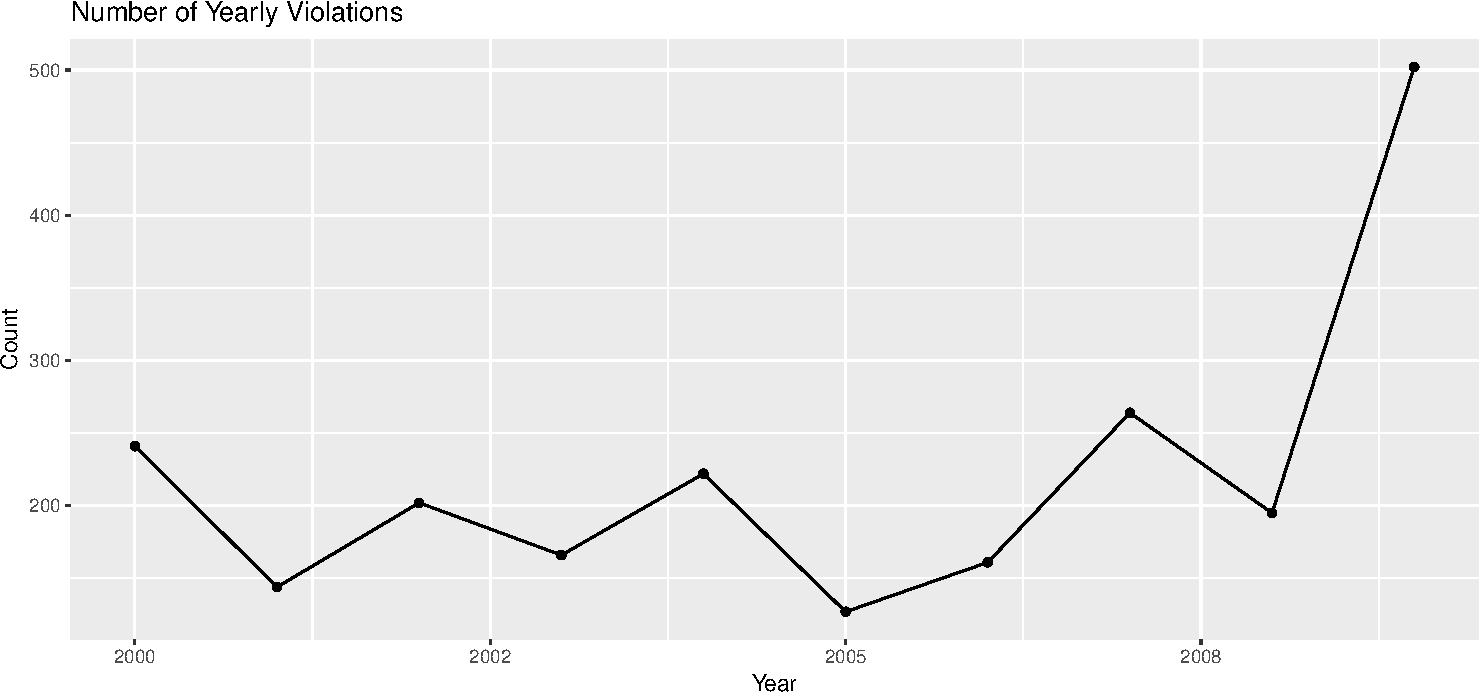
\includegraphics{presentation_slides_files/figure-beamer/upper big branch-1} \end{center}

\end{frame}

\begin{frame}{Violation Trend: Sago Mine}

\begin{center}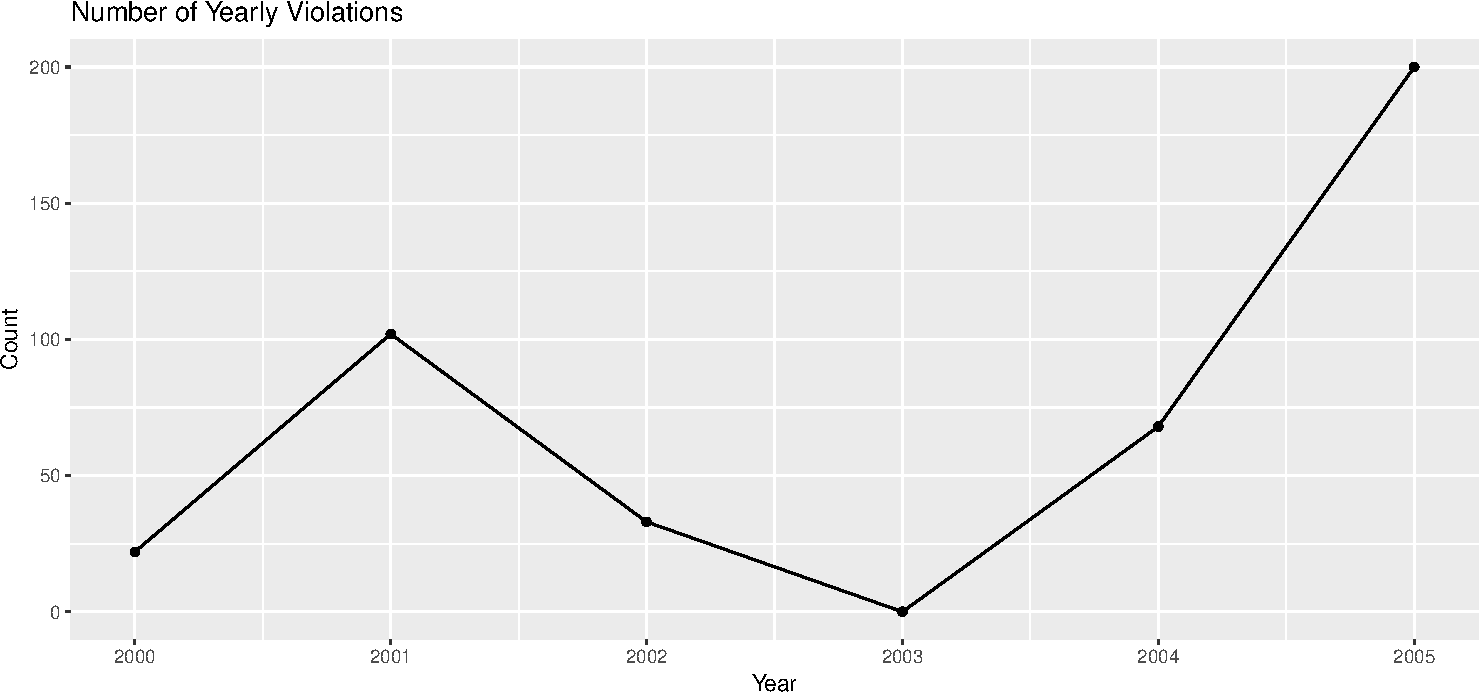
\includegraphics{presentation_slides_files/figure-beamer/sago-1} \end{center}

\end{frame}

\begin{frame}[fragile]{Predictive Model}

\begin{itemize}[<+->]
\tightlist
\item
  Rising violation trends before disasters
\item
  Develop a disaster classifier based on historical data
\item
  Define a \textbf{severe} accident as one with death or permenant
  disability 


\begin{verbatim}
## # A tibble: 2 × 3
##   severe      n  perc
##    <lgl>  <int> <dbl>
## 1  FALSE 477077 99.46
## 2   TRUE   2608  0.54
\end{verbatim}
\end{itemize}
\end{frame}

\begin{frame}[fragile]{Fixed-Mine Effects}

\begin{itemize}[<+->]
\tightlist
\item
  Biostatisticians and epidemiologists call it ``conditional logistic
  regression'' (\texttt{survival::clogit})
\item
  Suitable for \textbf{panel data} (e.g., longitudinal data, our
  consolidated data)
\item
  Model includes mine-specific biases
\item
  Logistic function (for every mine)


\[\Pr(Y=1|\mathbf{X}) = \frac{1}{1+e^{-(\alpha+\boldsymbol\beta\mathbf{X})}}\]


\item
  Logistic function with fixed effects (for the \(i\)-th mine)


\[\Pr(Y=1|\mathbf{X},i) = \frac{1}{1+e^{-(\alpha_i+\boldsymbol\beta\mathbf{x})}}\]
\end{itemize}

\end{frame}

\section{Results and Discussion}\label{results-and-discussion}

\begin{frame}[fragile]{Logistic Regression Without Fixed Effects}

\begin{itemize}[<+->]
\tightlist
\item
  In-sample model
%\end{itemize}

\begin{verbatim}
##           Reference
## Prediction  FALSE   TRUE
##      FALSE 477011   2600
##      TRUE      66      8
\end{verbatim}

\begin{verbatim}
##    Accuracy Sensitivity Specificity   Precision          F1 
##      0.9944      0.0031      0.9999      0.1081      0.0060
\end{verbatim}

%\begin{itemize}[<+->]
\tightlist
\item
  Accuracy = (TP + TN)/(P + N)
\item
  Sensitivity/recall = TP/P
\item
  Specificity = TN/N
\item
  Precision = TP/(TP + FP)
\item
  F1: harmonic mean of sensitivity and precision
\end{itemize}

\end{frame}

\begin{frame}[fragile]{Logistic Regression Without Fixed Effects}

\begin{itemize}[<+->]
\tightlist
\item
  Fails to predict top 10 deadliest disasters


\begin{verbatim}
##                      mine.name year quarter severe  pred
## 1  Upper Big Branch Mine-South 2010       2   TRUE FALSE
## 2                    Sago Mine 2006       1   TRUE FALSE
## 3         Crandall Canyon Mine 2007       3   TRUE FALSE
## 4              Darby Mine No 1 2006       2   TRUE FALSE
## 5                  Gibson Mine 2007       3   TRUE FALSE
## 6                Affinity Mine 2013       1   TRUE FALSE
## 7         Aracoma Alma Mine #1 2006       1   TRUE FALSE
## 8       Black Stallion UG Mine 2014       2   TRUE FALSE
## 9                Cucumber Mine 2007       1   TRUE FALSE
## 10             D-14 Stillhouse 2005       3   TRUE FALSE
\end{verbatim}
\end{itemize}
\end{frame}

\begin{frame}[fragile]{Logistic Regression Without Fixed Effects}

\begin{itemize}[<+->]
\tightlist
\item
  List of false positive predictions based on predicted probability 


\begin{verbatim}
##                                 mine.name year quarter severe pred
## 1  The American Coal Company New Era Mine 2008       3  FALSE TRUE
## 2  The American Coal Company New Era Mine 2008       2  FALSE TRUE
## 3  The American Coal Company New Era Mine 2007       4  FALSE TRUE
## 4  The American Coal Company New Era Mine 2008       4  FALSE TRUE
## 5  The American Coal Company New Era Mine 2008       1  FALSE TRUE
## 6  The American Coal Company New Era Mine 2009       1   TRUE TRUE
## 7  The American Coal Company New Era Mine 2007       3  FALSE TRUE
## 8  The American Coal Company New Era Mine 2006       1  FALSE TRUE
## 9  The American Coal Company New Era Mine 2005       4  FALSE TRUE
## 10 The American Coal Company New Era Mine 2006       2   TRUE TRUE
\end{verbatim}
\end{itemize}
\end{frame}

\begin{frame}[fragile]{Logistic Regression with Fixed Effects}

\begin{itemize}[<+->]
\tightlist
\item
  Out-of-sample model (randomly select half of the data to train and the
  other half to test)


\begin{verbatim}
##           Reference
## Prediction  FALSE   TRUE
##      FALSE 141332    483
##      TRUE   97167    852
\end{verbatim}

\begin{verbatim}
##    Accuracy Sensitivity Specificity   Precision          F1 
##      0.5928      0.6382      0.5926      0.0087      0.0172
\end{verbatim}
\end{itemize}
\end{frame}

\begin{frame}[fragile]{Logistic Regression with Fixed Effects}

\begin{itemize}[<+->]
\tightlist
\item
  Successfully predicts top 10 deadliest disasters


\begin{verbatim}
##                        mine.name year quarter severe pred
## 1                      Sago Mine 2006       1   TRUE TRUE
## 2           Crandall Canyon Mine 2007       3   TRUE TRUE
## 3                Darby Mine No 1 2006       2   TRUE TRUE
## 4                  Cucumber Mine 2007       1   TRUE TRUE
## 5                    Dotiki Mine 2010       2   TRUE TRUE
## 6                       Equality 2011       4   TRUE TRUE
## 7                    Meikle Mine 2010       3   TRUE TRUE
## 8            Nanuuq Gold Project 2007       3   TRUE TRUE
## 9  4 J's Gravel Crushing Plant 2 2011       3   TRUE TRUE
## 10                         Adams 2006       3   TRUE TRUE
\end{verbatim}
\end{itemize}
\end{frame}

\begin{frame}[fragile]{Logistic Regression with Fixed Effects}

\begin{itemize}[<+->]
\tightlist
\item
  Still has a lot of false positive predictions
\item
  List of false positive predictions based on predicted probability


\begin{verbatim}
##                                 mine.name year quarter severe pred
## 1  The American Coal Company New Era Mine 2006       1  FALSE TRUE
## 2             Upper Big Branch Mine-South 2009       3  FALSE TRUE
## 3             Upper Big Branch Mine-South 2009       1  FALSE TRUE
## 4             Upper Big Branch Mine-South 2006       4  FALSE TRUE
## 5             Upper Big Branch Mine-South 2005       1  FALSE TRUE
## 6  The American Coal Company New Era Mine 2005       3  FALSE TRUE
## 7  The American Coal Company New Era Mine 2008       1  FALSE TRUE
## 8  The American Coal Company New Era Mine 2007       4  FALSE TRUE
## 9             Upper Big Branch Mine-South 2006       1  FALSE TRUE
## 10            Upper Big Branch Mine-South 2006       3  FALSE TRUE
\end{verbatim}

%\begin{itemize}[<+->]
%\tightlist
\item
  What happened in the New Era Mine?
\end{itemize}

\end{frame}

\begin{frame}[fragile]{New Era Mine}

\begin{itemize}[<+->]
\tightlist
\item
  Among the worst mines by number of days lost due to accidents
%\end{itemize}

\begin{verbatim}
##                                 mine.name year quarter days.lost
## 1  The American Coal Company New Era Mine 2005       2      2940
## 2  The American Coal Company New Era Mine 2003       2      2914
## 3  The American Coal Company New Era Mine 2005       3      2874
## 4                                 Mathies 2002       1      2840
## 5  The American Coal Company New Era Mine 2004       3      2613
## 6  The American Coal Company New Era Mine 2004       1      2591
## 7                  Monongalia County Mine 2013       3      2563
## 8  The American Coal Company New Era Mine 2005       4      2487
## 9                     Powhatan No. 6 Mine 2013       1      2409
## 10                            Maple Creek 2001       1      2030
\end{verbatim}


%\begin{itemize}[<+->]
%\tightlist
\item
  Rising violation trend from 2000 to 2005
\end{itemize}

\end{frame}

\begin{frame}{New Era Mine}

\begin{center}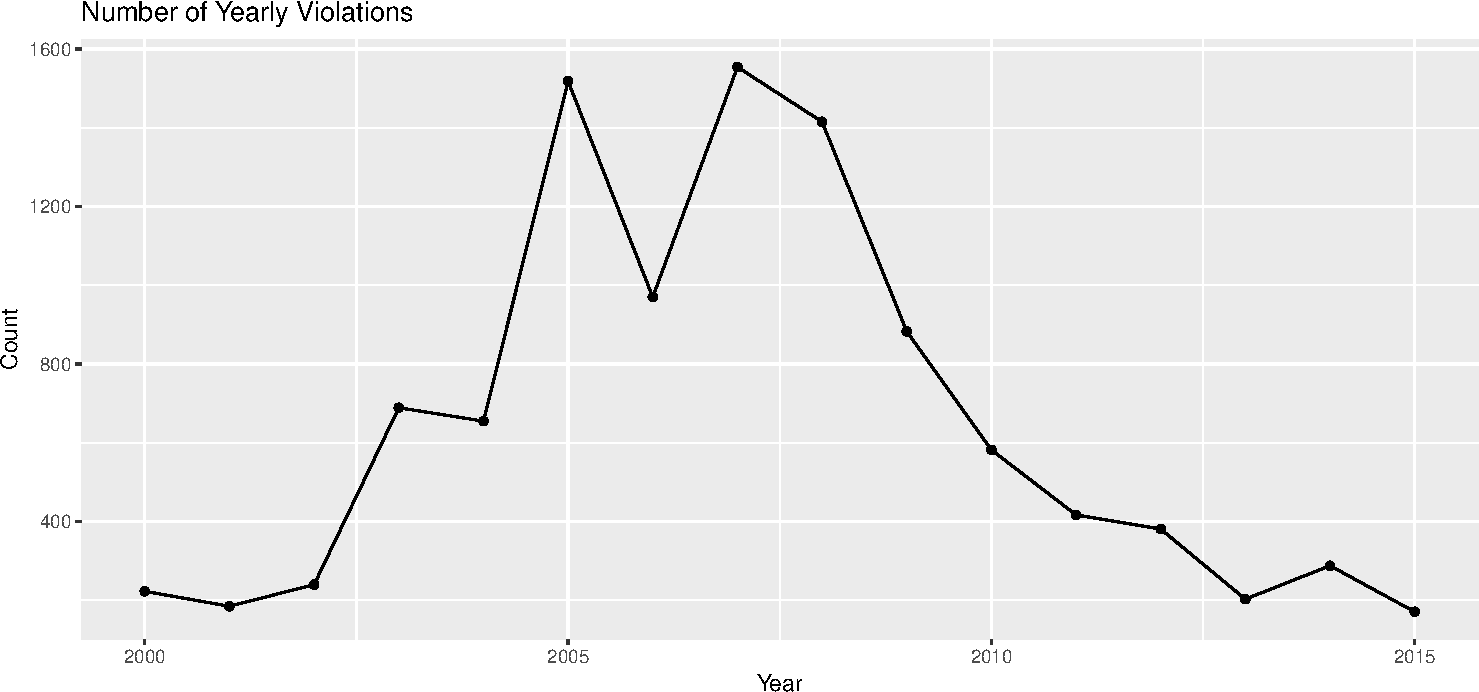
\includegraphics{presentation_slides_files/figure-beamer/new era viol-1} \end{center}

\end{frame}

\begin{frame}[fragile]{New Labels Including Days Lost}

\begin{itemize}[<+->]
\tightlist
\item
  Updated severe accident label

  \begin{itemize}[<+->]
  \tightlist
  \item
    Previously defined criteria plus days lost \(>\) 300
  \end{itemize}
\item
  Redo out-of-sample model
%\end{itemize}

\begin{verbatim}
##           Reference
## Prediction  FALSE   TRUE
##      FALSE 148496   1267
##      TRUE   88426   1645
\end{verbatim}

\begin{verbatim}
##    Accuracy Sensitivity Specificity   Precision          F1 
##       0.626       0.565       0.627       0.018       0.035
\end{verbatim}

%\begin{itemize}[<+->]
%\tightlist
\item
  Worse true positive rate, improved F1 score
\end{itemize}

\end{frame}

\begin{frame}[fragile]{New Labels Including Days Lost}

\begin{itemize}[<+->]
\tightlist
\item
  Successfully predicts 9 out of top 10 deadliest accidents


\begin{verbatim}
##                        mine.name year quarter severe  pred
## 1                      Sago Mine 2006       1   TRUE  TRUE
## 2           Crandall Canyon Mine 2007       3   TRUE  TRUE
## 3                Darby Mine No 1 2006       2   TRUE  TRUE
## 4                  Cucumber Mine 2007       1   TRUE  TRUE
## 5                    Dotiki Mine 2010       2   TRUE  TRUE
## 6                       Equality 2011       4   TRUE  TRUE
## 7                    Meikle Mine 2010       3   TRUE  TRUE
## 8            Nanuuq Gold Project 2007       3   TRUE  TRUE
## 9  4 J's Gravel Crushing Plant 2 2011       3   TRUE  TRUE
## 10                         Adams 2006       3   TRUE FALSE
\end{verbatim}
\end{itemize}
\end{frame}

\begin{frame}[fragile]{New Labels Including Days Lost}

\begin{itemize}[<+->]
\tightlist
\item
  Accidents of the New Era mine are now true positives


\begin{verbatim}
##                                 mine.name year quarter severe pred
## 1  The American Coal Company New Era Mine 2006       1   TRUE TRUE
## 2  The American Coal Company New Era Mine 2005       3   TRUE TRUE
## 3  The American Coal Company New Era Mine 2005       1   TRUE TRUE
## 4                  Monongalia County Mine 2014       3   TRUE TRUE
## 5                     Powhatan No. 6 Mine 2013       3   TRUE TRUE
## 6                     Powhatan No. 6 Mine 2013       4   TRUE TRUE
## 7                    Marshall County Mine 2015       4   TRUE TRUE
## 8  The American Coal Company New Era Mine 2008       1   TRUE TRUE
## 9                      Willow Lake Portal 2008       2   TRUE TRUE
## 10                    Powhatan No. 6 Mine 2013       1   TRUE TRUE
\end{verbatim}
\end{itemize}
\end{frame}

\section{Conclusion}\label{conclusion}

\begin{frame}{Conclusion}

\begin{itemize}[<+->]
\tightlist
\item
  Summary

  \begin{itemize}[<+->]
  \tightlist
  \item
    Two deadliest mine accidents in the last decade: Upper Big Branch \&
    Sago
  \item
    Rich MSHA data that need clean-up
  \item
    Supervised predictive model
  \end{itemize}
\item
  Application

  \begin{itemize}[<+->]
  \tightlist
  \item
    ``Credit score'' for mine safety
  \item
    Regulators, mines, stakeholders
  \end{itemize}
\item
  Future

  \begin{itemize}[<+->]
  \tightlist
  \item
    Improve model performance
  \item
    Unsupervised clustering, neural nets, etc.
  \item
    Expand data: OSHA, EPA, etc.
  \end{itemize}
\end{itemize}

\end{frame}

\begin{frame}[fragile]{Appendix: Simple Linear Model}

\begin{itemize}[<+->]
\tightlist
\item
  Adjusted \(R^2=0.36\)


\begin{verbatim}
##                           Estimate Std. Error t value Pr(>|t|)
## (Intercept)                 0.5243    0.06725     7.8  6.4e-15
## last.quarter.lost           0.0566    0.00179    31.6 2.9e-218
## last.year.lost              0.0724    0.00093    77.8  0.0e+00
## last.three.years.lost       0.0338    0.00032   105.6  0.0e+00
## last.quarter.restrict      -0.0173    0.00461    -3.8  1.7e-04
## last.year.restrict         -0.0123    0.00243    -5.1  3.9e-07
## last.three.years.restrict   0.0072    0.00085     8.4  3.8e-17
## last.quarter.viol           0.3083    0.01095    28.1 3.5e-174
## last.year.viol              0.1352    0.00490    27.6 2.1e-167
## last.three.years.viol      -0.0346    0.00141   -24.7 4.2e-134
## last.quarter.death         -5.7149    1.09783    -5.2  1.9e-07
## last.year.death            -3.6943    0.64330    -5.7  9.3e-09
## last.three.years.death     -0.5155    0.33261    -1.5  1.2e-01
\end{verbatim}
\end{itemize}
\end{frame}

\begin{frame}[fragile]{Appendix: Unsupervised Clustering}

\begin{itemize}[<+->]
\tightlist
\item
  Apply \(k\)-means clustering to consolidated data on all 20 features
\item
  3 clusters: \texttt{low}-risk, \texttt{mid}-risk, and
  \texttt{high}-risk
\item
  Selected cluster centers (omitting 17 features)


\begin{verbatim}
##      num.days.lost num.days.restrict num.death
## low            5.3               2.1    0.0013
## mid          100.5              18.6    0.0164
## high         508.4              32.7    0.0431
\end{verbatim}

%\begin{itemize}[<+->]
%\tightlist
\item
  Cluster sizes
%\end{itemize}

\begin{verbatim}
##         low   mid high
## size 465203 13299 1183
\end{verbatim}
\end{itemize}
\end{frame}

\begin{frame}[fragile]{Appendix: Markov Chain}

\begin{itemize}[<+->]
\tightlist
\item
  Overall transition matrix
%\end{itemize}

\begin{verbatim}
##        low   mid  high
## low  0.997 0.003 0.000
## mid  0.087 0.906 0.006
## high 0.000 0.072 0.928
\end{verbatim}

%\begin{itemize}[<+->]
%\tightlist
\item
  Steady-state distribution


\begin{verbatim}
##       low   mid  high
## [1,] 0.97 0.028 0.003
\end{verbatim}
\end{itemize}
\end{frame}

\end{document}